\documentclass{article}
\usepackage{amsmath}
\usepackage{amssymb}
\usepackage{graphicx}
\usepackage{hyperref}
\usepackage[version=4]{mhchem}


\begin{document}
\section*{Problem}
In parallelogram \(A B C D\), shown here, points \(E\) and \(F\) are the midpoints of side \(A B\) and \(B C\), respectively. \(A F\) meets \(D E\) at \(G\) and \(B D\) at \(H\). Find the area of quadrilateral \(B H G E\) if the area of \(A B C D\) is 60 .\\
(A) 10\\
(B) 9\\
(C) 8\\
(D) 7\\
(E) 5\\
\centering
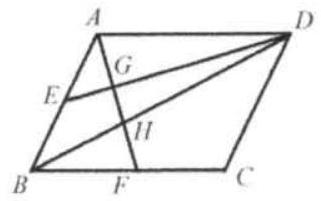
\includegraphics[width=\textwidth]{images/129(1).jpg}

\section*{Solution}
(D).\\
Extend \(A F\) and \(D C\) to meet at \(M\).


\(M C=A B=C D . A F=F M\).\\
Triangle \(A B H\) is similar to triangle \(M D H\).\\
\(\frac{A H}{H M}=\frac{A B}{D M}=\frac{1}{2}\)\\
\centering
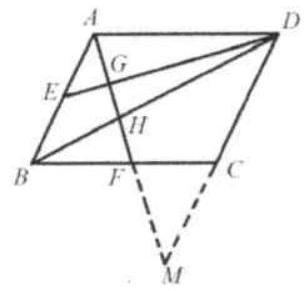
\includegraphics[width=\textwidth]{images/141(3).jpg}

Thus \(\frac{A H}{H M}=\frac{1}{3}\), and \(\frac{A H}{A F}=\frac{2}{3}\).\\
\(S_{\triangle A B H}=\frac{2}{3} S_{\triangle A B F}=\frac{2}{3} \times \frac{1}{4} S_{A B C D}=10\)\\
Triangle \(A E G\) is similar to triangle \(M D G\).\\
\centering
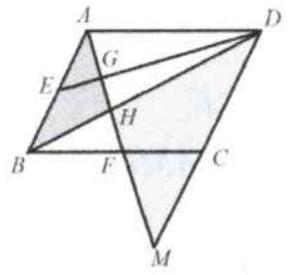
\includegraphics[width=\textwidth]{images/141.jpg}\\
\(\frac{E G}{D G}=\frac{A E}{M D}=\frac{1}{4}\). Thus \(\frac{E G}{E D}=\frac{1}{5}\).\\
\(S_{\triangle A E G}=\frac{1}{5} S_{\triangle A D E}=\frac{1}{5} \times \frac{1}{4} S_{A B C D}=3\).\\
Therefore \(S_{B H G E}=S_{\triangle A B H}-S_{\triangle A E G}=10-3=7\).\\
\centering
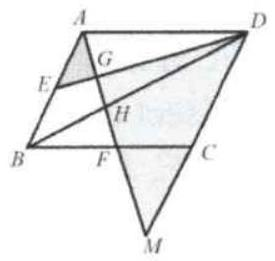
\includegraphics[width=\textwidth]{images/141(1).jpg}

\end{document}
